%% USTC thesis template ------------------------------------------
\documentclass[doctor, twoside, openany]{ustcthesis}
%% bachelor|master|doctor
%% 学位论文选项默认是 doctor
%%
%% chinese|english
%% 语种选项默认是 chinese
%%
%% 本科默认 oneside; 研究生默认 twoside, openany

%% Package -------------------------------------------------------
\usepackage{enumitem}
\setlist{nolistsep}
\setlist[enumerate,1]
  {labelindent=\parindent, leftmargin=*, label=\textup{(\arabic*)}}

\usepackage{amsmath,amssymb}
\usepackage{longtable,booktabs}
\bibliographystyle{plainnat}     % 参考文献格式
%\ctexset{chapter/fixskip=true}  % ctex 宏包 2016.06.03 引入的新选项, 修正章标题前的空白

%% Theorems ------------------------------------------------------
\usepackage{amsthm}
\def\proofname{\upshape\sffamily 证.}
\newtheoremstyle{ustctheorem}
  {\topsep}{\topsep}{\itshape}{}{\sffamily}{}{1em}{}
\newtheoremstyle{ustcdefinition}
  {\topsep}{\topsep}{}{}{\sffamily}{}{1em}{}

\theoremstyle{ustctheorem}
\newtheorem{theorem}{定理}[section]
\newtheorem{proposition}[theorem]{命题}
\newtheorem{lemma}[theorem]{引理}
\newtheorem{corollary}[theorem]{推论}

\theoremstyle{ustcdefinition}
\newtheorem{definition}[theorem]{定义}
\newtheorem{example}[theorem]{例}
\newtheorem{remark}[theorem]{注}

%% Title ---------------------------------------------------------
\title{中国科学技术大学\texorpdfstring{\\}{}本硕博毕业论文模板示例文档}
\author{赵钱孙}
\major{某}
\advisor{周吴郑~教授}
%\coadvisor{冯陈褚~教授}
%\date{\ctexset{today=big}\today}      % 默认是当前日期, 可手动修改
%\secrettext{机密\quad 小于等于20年}   % 内部|秘密|机密, 注释本行则不保密

\entitle{An Example of USTC Thesis Template for Bachelor, Master and Doctor}
\enauthor{Qiansun Zhao}
\enmajor{Whatever}
\enadvisor{Prof.~Wuzheng Zhou}
%\encoadvisor{Prof.~Chenchu Feng}
%\endate{\ctexset{today=old}\today}    % default is today
%\ensecrettext{Confidential\quad Less than or equal to 20 years}  % Internal|Secret|Confidential

%% ---------------------------------------------------------------

%\overfullrule10pt
\begin{document}

\maketitle

%% ---------------------------------------------------------------
%%
%% 本科生论文文档顺序:
%%   frontmatter: 致谢、目录、中文摘要、英文摘要
%%   mainmatter:  正文章节、参考文献
%%   appendix:    附录
%%
%% 研究生论文文档顺序:
%%   frontmatter: 中文摘要、英文摘要、目录、符号说明
%%   mainmatter:  正文、参考文献
%%   appendix:    附录
%%   backmatter:  致谢、发表论文
%%
%% ---------------------------------------------------------------
%%
%% 这里是按研究生论文的顺序安排的
%% 本科生论文请自行调整顺序
%%
%% ---------------------------------------------------------------

\frontmatter


\begin{abstract}
本文档是中国科学技术大学学位论文 \LaTeX{} 模板的一个示例文档. 这里会给出模板使用方法的简介. 模板选项及详细用法请参考说明文档 \verb|ustcthesis.pdf|.

\keywords{中国科学技术大学, 学位论文, \LaTeX{} 模板.}

\end{abstract}

\begin{enabstract}

This is a sample document of USTC thesis \LaTeX{} template. This document will show the usage of the template. For more information, please refer to the template document \verb|ustcthesis.pdf|.

\enkeywords{University of Science and Technology of China (USTC), Thesis, \LaTeX{} Template.}

\end{enabstract}
\tableofcontents
\listoffigures
\listoftables
\begin{notation}

\begin{tabbing}

  \hspace*{8em}\=\kill

  \textsf{集合} \\
  $\emptyset$  \> 空集 \\
  $\in$        \> 属于 \\
  $\subseteq$  \> 包含于 \\
  $\cap$       \> 交 \\
  $\cup$       \> 并 \\[\baselineskip]

  \textsf{数集} \\
  $\mathbb{N}$ \> 自然数集 \\
  $\mathbb{Z}$ \> 整数集 \\
  $\mathbb{Q}$ \> 有理数集 \\
  $\mathbb{R}$ \> 实数集 \\
  $\mathbb{C}$ \> 复数集 \\

\end{tabbing}

\end{notation}


\mainmatter

\chapter{绪论 (Introduction)}

\verb|ustcthesis| 是用于排版中国科学技术大学学位论文的 \LaTeX{} 模板. 适用于学士, 硕士和博士的学位论文编写. 由 jiaopjie 参照《中国科学技术大学研究生学位论文撰写规范》
\footnote{\url{http://gradschool.ustc.edu.cn/ylb/material/xw/wdxz/1.doc}}
和《关于本科毕业论文(设计)格式和统一封面的通知》
\footnote{\url{http://www.teach.ustc.edu.cn/document/doc-administration/4032.html}}
的要求编写. 本模板的编写过程中参考了已有的论文模板的编写方式.

早期的模板有中国科学技术大学本科论文模板 (作者XPS, 最后维护ywg)
\footnote{\url{https://github.com/ywgATustcbbs/ustcthesis.bachelor}}
和中国科学技术大学研究生论文模板 (作者Liuqs,主要维护Liuqs, Guolicai)
\footnote{\url{https://github.com/ywgATustcbbs/ustcthesis.msphd}}.
后来 ywg@USTC 对这两个模板进行了整合梳理并对其维护
\footnote{\url{https://github.com/ywgATustcbbs/ustcthesis}}.
该模板在研究生院网站和 bbs 站点均有下载链接. 2015 年, seisman 和 zepinglee 基于 \verb|ctex| 2.0 重新编写了模板
\footnote{\url{https://github.com/ustctug/ustcthesis}}.

ywg@USTC 整合后的模板有不少冗余代码. 该模板自 2016 年 2 月以来尚未更新. 并且在 TeXLive 2016 下, 该模板中的 \verb|appendix| 环境会报错. 而 seisman 和 zepinglee 写的模板中, 制作扉页时用了 \verb|tikz| 宏包. 不少写法个人不喜欢. 鉴于此我决定写个模板自用, 顺便把自己的编写思路记录下来. 因此本模板仅保证基本的格式要求. 额外的需求请自行使用相应的宏包.

\chapter{说明}
\label{chap:readme}

注意到《中国科学技术大学研究生学位论文撰写手册》中的格式要求有矛盾的地方.
这里适当作了一些调整.

\section{注意事项}

使用本模板之前请注意以下事项.

\begin{itemize}
  \item
    扉页中各项目与页面上边缘的距离作了调整.
  \item
    两到四字的章标题 (包括目录、摘要、致谢等), 字中间没有留空白.
  \item
    没有处理参考文献列表的格式. 请自行使用合适的 \verb|.bst| 格式文件.
  \item
    默认未开启伪粗体.
  \item
    模板支持使用 XeLaTeX 或者 LuaLaTeX 编译
    (推荐使用 XeLaTeX, 使用 LuaLaTeX 时不支持开启伪粗体).
  \item
    使用前请升级宏包. 其中 \verb|ctex| 宏包应该升级到 2.0 版本以上.
\end{itemize}

\section{文档选项}

模板新设置了一些文档选项, 如\autoref{tab:doc-option} 所示.

\begin{table}[!htb]
  \caption{模板的文档选项}
  \label{tab:doc-option}
  \centering
  \begin{tabular}{ll}
    \toprule
    选项                & 说明\\
    \midrule
    \verb|doctor|       & 博士学位 (默认)\\
    \verb|master|       & 硕士学位\\
    \verb|bachelor|     & 学士学位\\
    \midrule
    \verb|chinese|      & 中文论文 (默认)\\
    \verb|english|      & 英文论文\\
    \midrule
    \verb|academic|     & 学术学位 (默认)\\
    \verb|professional| & 专业学位\\
    \bottomrule
  \end{tabular}
\end{table}

另外, \verb|book| 文档类提供的文档选项仍然可用.
模板更改了其中 \verb|openright| 和 \verb|openany| 选项的默认值,
参见\autoref{tab:book-option}.

\begin{table}[!htb]
  \caption{单双面选项}
  \label{tab:book-option}
  \centering
  \begin{tabular}{lp{16em}l}
    \toprule
    选项             & 说明\\
    \midrule
    \verb|oneside|   & 单面格式\\
    \verb|twoside|   & 双面格式 (默认)\\
    \midrule
    \verb|openright| & 双面格式下新一章总是从奇数页开始\\
    \verb|openany|   & 双面格式下新一章总是从新一页开始
                       (双面格式下默认)\\
    \bottomrule
  \end{tabular}
\end{table}

\section{字体设置}

模板的中文字体由 \verb|ctex| 宏包自动设置.
以下几点需要注意.

\begin{itemize}
  \item
    较新的 Windows 系统下默认的微软雅黑可能不太适合打印.
  \item
    其他系统可能会缺少一些字体, 如仿宋、隶书以及 Times New Roman 等.
  \item
    \verb|ctex| 宏包默认不开启伪粗体, 此时宋体的加粗一般用黑体代替.
\end{itemize}

用户可以自定义文档字体.
相关命令可参见\autoref{tab:font-set}.
自定义字体时可通过 \verb|BoldFont| 选项设定粗体的替代字体
(或通过 \verb|AutoFakeBold| 选项开启伪粗体),
通过 \verb|ItalicFont| 选项设定斜体的替代字体.

\begin{table}[!htb]
  \caption{自定义字体命令}
  \label{tab:font-set}
  \centering
  \begin{tabular}{ll}
    \toprule
    命令                   & 说明\\
    \midrule
    \verb|\setmainfont|    & 设置衬线字体\\
    \verb|\setsansfont|    & 设置无衬线字体\\
    \verb|\setmonofont|    & 设置等宽字体\\
    \midrule
    \verb|\setCJKmainfont| & 设置中文衬线字体\\
    \verb|\setCJKsansfont| & 设置中文无衬线字体\\
    \verb|\setCJKmonofont| & 设置中文等宽字体\\
    \bottomrule
  \end{tabular}
\end{table}

下面针对 Windows 系统提供几点解决方案.

\begin{enumerate}
  \item
    使用 Fandol 字体 (比较容易缺字), 或者自行下载有粗体形式的字体
    (如思源字体). 可如下设置 (斜体用楷体代替).
\begin{verbatim}
\setCJKmainfont[ItalicFont={KaiTi}]{Source Han Serif SC}
\setCJKsansfont[ItalicFont={KaiTi}]{Source Han Sans SC}
\end{verbatim}
  \item
    使用中易字体, 并开启伪粗体. 伪粗体一般被认为质量比较差, 慎用.
\begin{verbatim}
\setCJKmainfont[AutoFakeBold=3,ItalicFont={KaiTi}]{SimSun}
\setCJKsansfont[AutoFakeBold=3,ItalicFont={KaiTi}]{SimHei}
\end{verbatim}
  \item
    使用中易黑体替换微软雅黑, 且关闭伪粗体.
    宋体的加粗形式一般是使用黑体代替.
\begin{verbatim}
\setCJKsansfont[ItalicFont={KaiTi}]{SimHei}
\end{verbatim}
    这种情况下, 中英混排会有以下两个小问题.
    \begin{itemize}
      \item
        黑体加粗时 (如扉页中的文章标题和\Emph{研究生论文}的章标题),
        中文不加粗, 而英文加粗, 稍微欠协调.
      \item
        宋体加粗时 (如\Emph{研究生论文}的插图和表格标题),
        中文是黑体, 而英文是加粗的 Times New Roman, 稍微欠协调.
    \end{itemize}
    用户可自行把相应的标题都修改为黑体不加粗.
    这主要包括中英文标题、章标题、插图和表格标题、“关键词”字样.
    其中, 中英文标题不加粗, 可在 \verb|\title| 和 \verb|\entitle| 的参数中
    加上 \verb|\mdseries|.
\begin{verbatim}
\ctexset{chapter={format+=\mdseries}}
\captionsetup{font+={md,sf}}
\entitle{\mdseries <English title>}
\end{verbatim}
\end{enumerate}

\section{扉页}

扉页中各项目与页面上边缘的距离作了调整.
下面是一些注意事项.

\begin{itemize}
  \item
    扉页所需的个人信息由\autoref{tab:info} 中命令设置, 它们应该用在导言区.
  \item
    若导师多于一人, 请一并用 \verb|\supervisor| 和 \verb|\ensupervisor| 给出.
  \item
    若英文专业或导师的文本过长, 可用 \verb|\\| 在合适的地方换行.
  \item
    扉页由命令 \verb|\maketitle| 生成, 它应该作为正文开始后的第一个命令.
  \item
    默认日期为当前日期.
\end{itemize}

\begin{table}[!htb]
  \caption{个人信息命令}
  \label{tab:info}
  \centering
  \begin{tabular}{lll}
    \toprule
    命令            & 命令 (英文)       & 说明\\
    \midrule
    \verb|\title|        & \verb|\entitle|        & 论文标题\\
    \verb|\author|       & \verb|\enauthor|       & 作者姓名\\
    \verb|\major|        & \verb|\enmajor|        & 学科专业\\
    \verb|\supervisor|   & \verb|\ensupervisor|   & 导师姓名\\
    \verb|\date|         & \verb|\endate|         & 完成日期\\
    \verb|\secrettext|   & \verb|\ensecrettext|   & 密级信息\\
    \bottomrule
  \end{tabular}
\end{table}

\verb|ctex| 宏包汉化了 \verb|\today| 命令,
并提供了 \verb|small|, \verb|big|, \verb|old| 三种样式.
\begin{itemize}
  \item \verb|small| 中文样式, 其中数字使用阿拉伯数字.
  \item \verb|big| 全汉字样式.
  \item \verb|old| 原英文样式
\end{itemize}
\verb|ctex| 默认的是 \verb|small| 样式. \verb|\ctexset{today=old}| 则切换到英文日期样式.

\section{模板提供的环境}

本模板对中英文摘要、符号说明、致谢、研究成果部分提供了专门的环境,
如\autoref{tab:doc-environment} 所示.
这主要是因为这些部分的格式要求与普通章的格式略有区别.

如果不在意这种区别的话, 完全可以用 \verb|\chapter*| 甚至 \verb|\chapter| 命令来代替.
例如 \verb|\chapter{摘要}|, \verb|\chapter{符号说明}|.

\begin{table}[!htb]
  \caption{模板提供的环境}
  \label{tab:doc-environment}
  \centering
  \begin{tabular}{ll}
    \toprule
    环境或命令              & 说明\\
    \midrule
    \verb|abstract|         & 中文摘要\\
    \verb|enabstract|       & 英文摘要\\
    \verb|notation|         & 符号说明\\
    \verb|acknowledgements| & 致谢\\
    \verb|publications|     & 研究成果\\
    \midrule
    \verb|\keywords|        & 中文关键词 (用在 \verb|abstract| 环境中)\\
    \verb|\enkeywords|      & 英文关键词 (用在 \verb|enabstract| 环境中)\\
    \bottomrule
  \end{tabular}
\end{table}

\section{图片和表格}

图片和表格很类似, 都可以混排的正文中, 也都可以放入对应的浮动体环境.
需要注意的是, 浮动体中 \verb|\caption| 命令应该置于 \verb|\label| 命令之前.

对于尺寸较小的图片和表格, 排版安排可以稍微随意一些.
即使混排在正文中也不会带来糟糕的影响.
比如\autoref{sec:bib}中没有表头的小表格就是用 \verb|center| 环境混排在正文中.

对于占用空间较大的图片和表格, 则应该放入对应的浮动体环境 \verb|figure| 和 \verb|table| 中.
这两个环境均可以带位置选项 \verb|h, t, b, p| 分别对应当前位置、页面顶端、页面底部、独占一页.
可以使用 \verb|!| 表示相对更靠近当前位置.

\subsection{图片}

\LaTeX{} 可以插入各种常见格式的图片.

\autoref{fig:test} 放在了浮动环境 \verb|figure| 中.
由于占用空间很小, 它很有可能就在下面.

\begin{figure}[!htb]
\centering
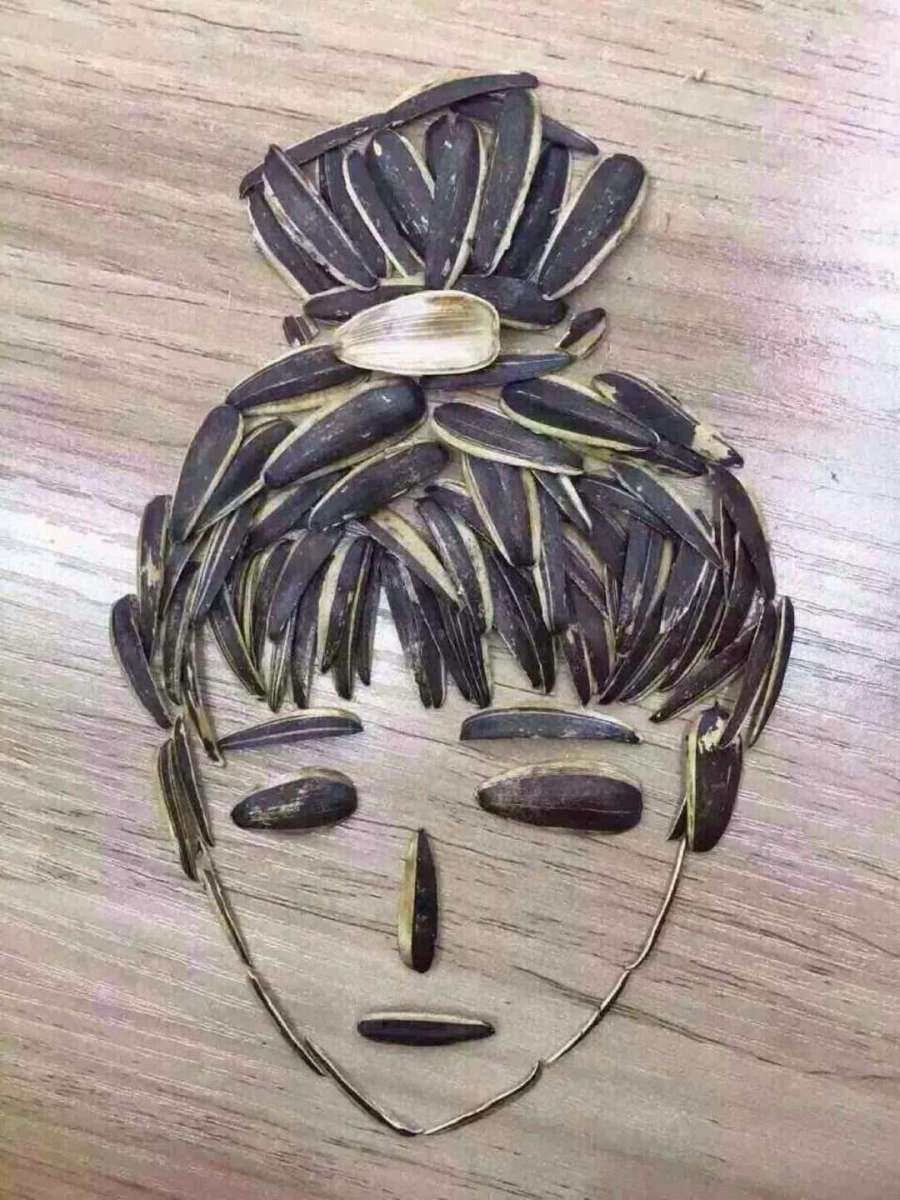
\includegraphics[height=3cm]{figure/test}
\caption{测试图片}
\label{fig:test}
\captionnote{这是个小图片. 该图片来自网络, 请勿用于商业用途.}
\end{figure}

\autoref{fig:test-big} 放在了浮动环境 \verb|figure| 中.
但由于占用空间较大, 它很有可能会跑到其他地方去了.

\begin{figure}[!htbp]
\centering
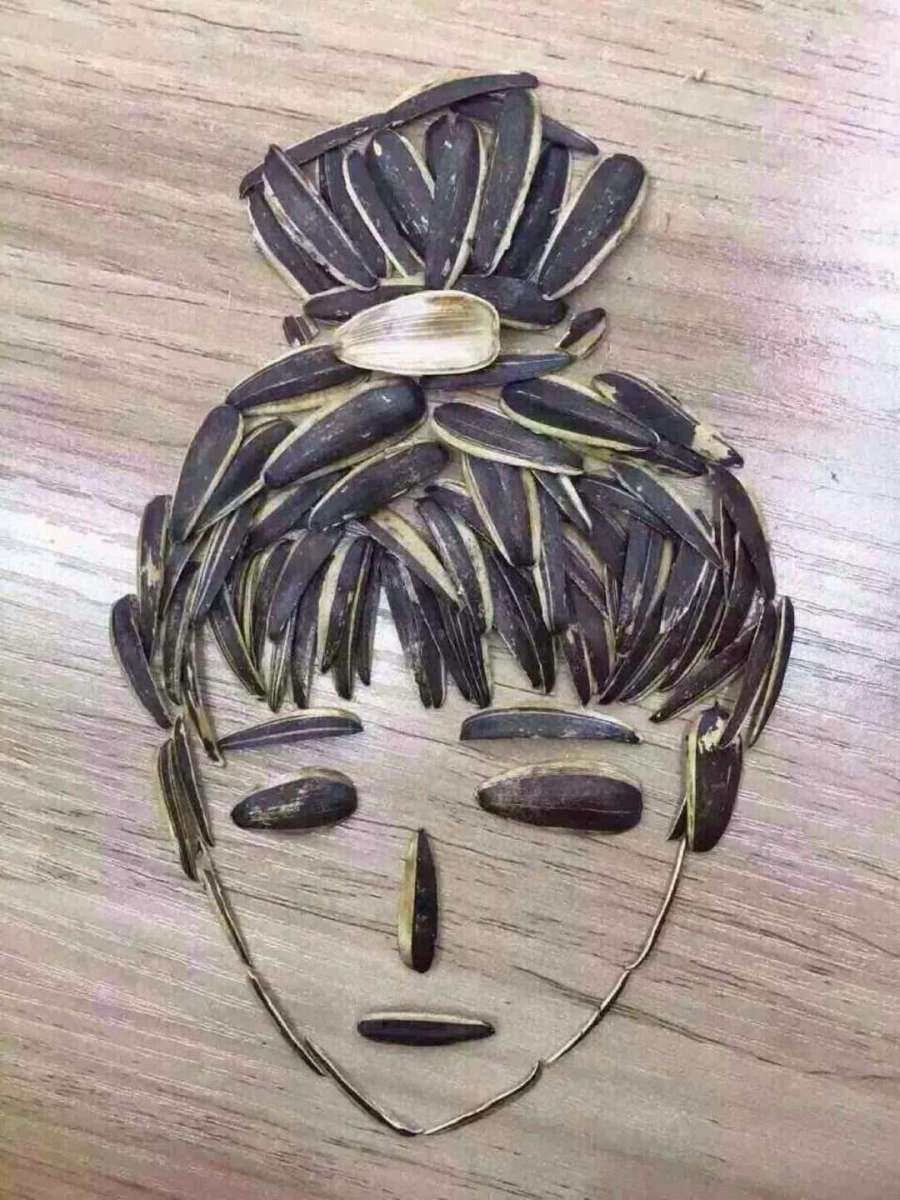
\includegraphics[width=8cm]{figure/test}
\caption{尺寸较大的图片}
\label{fig:test-big}
\captionnote{这是个尺寸较大的图片. 该图片放在了 \texttt{figure} 浮动环境中. 它的位置可以浮动. 它很有可能不会出现在代码所在的位置. 由于使用了 \texttt{p} 选项, 它很有可能独占了一页. 该图片来自网络, 请勿用于商业用途.}
\end{figure}

\subsection{表格}

\autoref{tab:test} 放在了浮动环境 \verb|table| 中.
由于占用空间很小, 它很有可能就在下面.

\begin{table}[!htb]
  \caption{普通表格}
  \label{tab:test}
  \centering
  \begin{tabular}{ccc}
    \toprule
    左 & 中 & 右\\
    \midrule
    1  & a  & b\\
    2  & a  & b\\
    3  & a  & b\\
    \bottomrule
  \end{tabular}
  \captionnote{这是个普通表格.}
\end{table}

\section{参考文献}
\label{sec:bib}

参考文献引用部分使用了 \verb|natbib| 宏包.
该宏包修改了 \verb|\cite| 命令, 并提供了新命令 \verb|\citet| 和 \verb|\citep|.

\verb|natbib| 宏包提供了两种引用模式: author-year 和 numerical.
它们可分别使用 \verb|authoryear| 和 \verb|numbers| 选项激活.
numerical 模式还有上标的形式, 可由 \verb|super| 选项激活.
其中 \verb|authoryear| 为默认选项.

宏包预定义了圆括号和方括号两种定界符, 分别使用 \verb|round| 和 \verb|square| 选项激活.
其中 \verb|round| 为默认选项.

本模板载入该宏包时使用了 \verb|numbers| 和 \verb|square| 选项.

命令 \verb|\bibliographystyle| 用于指定参考文献的样式. 它的参数是要使用参考文献样式对应的 \verb|.bst| 文件的文件名 (不包括扩展名). 宏包 \verb|natbib| 的作者提供了三个可用于 \verb|authoryear| 模式的 \verb|.bst| 文件: \verb|plainnat.bst|, \verb|abbrvnat.bst|, \verb|unsrtnat.bst|.

需要注意的是, 一些标准的 \verb|.bst| 文件 (如 \verb|plain.bst|) 只支持 numerical 模式.
在 author-year 模式下使用这些文件格式可能会遇到下述的错误信息.\\
\verb|Bibliography not compatible with author-year citations.|\\
此时只使用 numerical 模式即可.

如果使用的 \verb|.bst| 文件支持 author-year 模式,
在行文中是可以随时通过 \verb|\setcitestyle| 命令切换引用模式的.
\begin{itemize}
  \item
    \verb|\setcitestyle{authoryear,round}| 切换到 author-year 模式,
    并选定圆括号作为定界符.
  \item
    \verb|\setcitestyle{numbers,square}| 切换到 numerical 模式,
    并选定方括号作为定界符.
  \item
    \verb|\setcitestyle{super}| 切换到上标的 numerical 模式,
    不更改定界符.
\end{itemize}

研究生论文撰写手册要求, 对多作者的文献进行缩写时区分中英文文献的缩写词后缀. 这可能需要自己编写新的 \verb|.bst| 文件. 用户如有这样的要求的话, 可自行编写或下载满足条件的 \verb|.bst| 文件
\footnote{例如: \url{https://github.com/ustctug/gbt-7714-2015}}.

\subsection{numerical 模式}

命令 \verb|\setcitestyle{numbers,square}| 切换到 numerical 模式, 并选定方括号作为定界符.
此时三个引用命令的效果如下表所示.

\setcitestyle{numbers,square}
\begin{center}
  \begin{tabular}{ll}
    \toprule
    命令                      & 效果\\
    \midrule
    \verb|\cite{Knuth1986a}|  & \cite{Knuth1986a}\\
    \verb|\citet{Knuth1986a}| & \citet{Knuth1986a}\\
    \verb|\citep{Knuth1986a}| & \citep{Knuth1986a}\\
    \bottomrule
  \end{tabular}
\end{center}

在 \verb|natbib| 宏包中, 这些引用命令都有两个可选参数, 分别是引用的前缀和后缀.
例如, 命令 \verb|\cite| 在 \verb|numbers| 模式下的效果如下.\\
\verb|\cite[参见][第~1~章]{Knuth1986a}|
$\Rightarrow$
\cite[参见][第~1~章]{Knuth1986a}

\subsection{上标的 numerical 模式}

命令 \verb|\setcitestyle{super}| 切换到上标的 numerical 模式, 不更改定界符.
此时三个引用命令的效果如下表所示.

\setcitestyle{super}
\begin{center}
  \begin{tabular}{ll}
    \toprule
    命令                      & 效果\\
    \midrule
    \verb|\cite{Knuth1986a}|  & \cite{Knuth1986a}\\
    \verb|\citet{Knuth1986a}| & \citet{Knuth1986a}\\
    \verb|\citep{Knuth1986a}| & \citep{Knuth1986a}\\
    \bottomrule
  \end{tabular}
\end{center}

\subsection{author-year 模式}

命令 \verb|\setcitestyle{authoryear,round}| 切换到 author-year 模式, 并选定圆括号作为定界符.
此时三个引用命令的效果如下表所示.

\setcitestyle{authoryear,round}
\begin{center}
  \begin{tabular}{ll}
    \toprule
    命令                      & 效果\\
    \midrule
    \verb|\cite{Knuth1986a}|  & \cite{Knuth1986a}\\
    \verb|\citet{Knuth1986a}| & \citet{Knuth1986a}\\
    \verb|\citep{Knuth1986a}| & \citep{Knuth1986a}\\
    \bottomrule
  \end{tabular}
\end{center}

引用命令在 author-year 模式下会对多作者的文献使用 ``author1 et al.'' 的形式进行缩写.
而带星号的引用命令则会罗列所有作者. 这些命令也都可以一次引用多个文献.
使用效果参见\autoref{tab:cite-multi-author}.

\begin{table}[!htb]
  \caption{文献引用效果}
  \label{tab:cite-multi-author}
  \centering
  \begin{tabular}{lp{0.45\textwidth}l}
    \toprule
    命令                                   & 效果\\
    \midrule
    \verb|\cite{Mittelbach2004}|           & \cite{Mittelbach2004}\\
    \verb|\cite*{Mittelbach2004}|          & \cite*{Mittelbach2004}\\
    \verb|\cite{Knuth1984,Knuth1986a}|     & \cite{Knuth1984,Knuth1986a}\\
    \verb|\cite{Knuth1984,Mittelbach2004}| & \cite{Knuth1984,Mittelbach2004}\\
    \verb|\cite{Liu2013,Deng2001}|         & \cite{Liu2013,Deng2001}\\
    \bottomrule
  \end{tabular}
\end{table}

我们指出以下两点注意事项.
\begin{itemize}
  \item
    如果行文中使用了 author-year 模式, 则在 \verb|\bibliography| 命令之前应该切换回 numerical 模式. 否则参考文献列表前面不会有数字编号的前缀.
  \item
    如果使用了 \verb|.bib| 文件生成参考文献列表, 则列表中的每一条文献都需要在正文中使用 \verb|\cite| 等命令引用. 否则应该使用命令 \verb|\nocite| 声明.
\end{itemize}

\chapter{测试 (Test)}\label{chap:test}

第一段\\
这是第二行\\
这是第三行\\
这是第四行\\
这是第五行.

第二段\\
这是第二行\\
这是第三行\\
这是第四行\\
这是第五行.

第三段\\
这是第二行\\
这是第三行\\
这是第四行\\
这是第五行.

第四段\\
这是第二行\\
这是第三行\\
这是第四行\\
这是第五行.

第五段\\
这是第二行\\
这是第三行\\
这是第四行\\
这是第五行.

第六段\\
一二三四五六七八九十一二三四五六七八九十一二三四五六七八九十一二三四五六七八九十一二三四五六七八九十一二三四五六七八九十一二三四五六七八九十一二三四五六七八九十一二三四五六七八九十一二三四五六七八九十一二三四五六七八九十一二三四五六七八九十一二三四五六七八九十.

第七段\\
一二三四五六七八九十一二三四五六七八九十一二三四五六七八九十一二三四五六七八九十一二三四五六七八九十一二三四五六七八九十一二三四五六七八九十一二三四五六七八九十一二三四五六七八九十一二三四五六七八九十一二三四五六七八九十一二三四五六七八九十一二三四五六七八九十.

第八段\\
一二三四五六七八九十一二三四五六七八九十一二三四五六七八九十一二三四五六七八九十一二三四五六七八九十一二三四五六七八九十一二三四五六七八九十一二三四五六七八九十一二三四五六七八九十一二三四五六七八九十一二三四五六七八九十一二三四五六七八九十一二三四五六七八九十.

第九段\\
这是第二行\\
这是第三行\\
这是第四行\\
这是第五行.

第十段\\
这是第二行\\
这是第三行\\
这是第四行\\
这是第五行.

\chapter{图片和表格}

\section{图片}

图~\ref{fig:test} 是个小图片. 因此尽管它在浮动环境中, 却很有可能就在下面.

\begin{figure}[!htb]
\centering

\includegraphics[width=4cm]{logo/ustc_logo_fig}
\caption{测试图片}
\label{fig:test}
\captionnote{这是个小图片}
\end{figure}

图~\ref{fig:bigfigure} 是一张尺寸比较大的图片. 再加上这个图片是在一个浮动环境中, 因此它很有可能会跑到其他地方去.

\begin{figure}[!htb]
\centering

\includegraphics[width=10cm]{logo/ustc_logo_fig}
\caption{这是个比较大的图片}
\label{fig:bigfigure}
\captionnote{This is a long caption note. This is a long caption note. This is a long caption note. This is a long caption note. This is a long caption note. This is a long caption note.}
\end{figure}

\section{普通表格}

表~\ref{tab:test} 是个小表格. 因此尽管它在浮动环境中, 却很有可能就在下面.

\begin{table}[!htb]
  \caption{普通表格}
  \label{tab:test}
  \centering
  \begin{tabular}{ccc}
    \toprule
    左 & 中 & 右\\
    \midrule
    1  & a  & b\\
    2  & a  & b\\
    3  & a  & b\\
    4  & a  & b\\
    5  & a  & b\\
    \bottomrule
  \end{tabular}
  \captionnote{这是个普通表格}
\end{table}

\section{长表格}

表~\ref{tab:longtable} 是一个长表格. 长表格似乎不能放在浮动环境中. 因此, 它的位置会是准确的.

\begin{center}
  \begin{longtable}{cccc}
    \caption{长表格}\label{tab:longtable}\\ % 首页的表序
    \toprule
    左 & 中 & 中 & 右\\
    \midrule
    \endfirsthead  % 到这里为止是首页的表头
    \caption[]{长表格 (续)}\\ % 后续页的表序
    \toprule
    左 & 中 & 中 & 右\\
    \midrule
    \endhead  % 到这里为止是后续页的表头
    \hline
    \multicolumn{4}{r}{\small 续下页}
    \endfoot  % 到这里为止是首页的表尾
    \bottomrule
    \captionnote{这是个长表格}
    \endlastfoot  % 到这里为止是后续页的表尾
    1  &  abc  &  def  &  xyz \\
    2  &  abc  &  def  &  xyz \\
    3  &  abc  &  def  &  xyz \\
    4  &  abc  &  def  &  xyz \\
    5  &  abc  &  def  &  xyz \\
    6  &  abc  &  def  &  xyz \\
    7  &  abc  &  def  &  xyz \\
    8  &  abc  &  def  &  xyz \\
    9  &  abc  &  def  &  xyz \\
    10 &  abc  &  def  &  xyz \\
    11 &  abc  &  def  &  xyz \\
    12 &  abc  &  def  &  xyz \\
    13 &  abc  &  def  &  xyz \\
    14 &  abc  &  def  &  xyz \\
    15 &  abc  &  def  &  xyz \\
    16 &  abc  &  def  &  xyz \\
    17 &  abc  &  def  &  xyz \\
    18 &  abc  &  def  &  xyz \\
    19 &  abc  &  def  &  xyz \\
    20 &  abc  &  def  &  xyz \\
    21 &  abc  &  def  &  xyz \\
    22 &  abc  &  def  &  xyz \\
    23 &  abc  &  def  &  xyz \\
    24 &  abc  &  def  &  xyz \\
    25 &  abc  &  def  &  xyz \\
    26 &  abc  &  def  &  xyz \\
    27 &  abc  &  def  &  xyz \\
    28 &  abc  &  def  &  xyz \\
    29 &  abc  &  def  &  xyz \\
    30 &  abc  &  def  &  xyz \\
    31 &  abc  &  def  &  xyz \\
    32 &  abc  &  def  &  xyz \\
    33 &  abc  &  def  &  xyz \\
    34 &  abc  &  def  &  xyz \\
    35 &  abc  &  def  &  xyz \\
  \end{longtable}
\end{center}

\chapter{定理环境}

\chapter{引用}

\section{自动引用}

自动引用可以由 \verb|hyperref| 宏包提供的命令 \verb|\autoref| 来实现. 自动引用会在引用标号前自动加上对应的前缀. 并且会把前缀和标号一起加上超链接. 效果如下.

定理~\ref{thm:test}. \autoref{def:test}. \autoref{lem:test}. \autoref{prop:test}. \autoref{thm:test}. \autoref{rem:test}. \autoref{ex:test}. \autoref{cor:test}. \autoref{fig:test}. \autoref{tab:test}. \autoref{eq:test}. \autoref{chap:test}.

由于这里各种定理环境共用一个计数器, 自动引用的前缀都是 ``定理''. 若要对不同定理环境区分前缀, 可通过宏包 \verb|aliascnt| 对 \verb|hyperref| 宏包做一些修正.

\section{文献引用}

参考文献引用部分使用了 \verb|natbib| 宏包. 该宏包提供了两种引用文献模式: author-year 和 numerical. 载入该宏包时使用了 \verb|numbers| 选项.

命令 \verb|\bibliographystyle| 用于指定参考文献的样式. 它的参数是要使用参考文献样式对应的 \verb|.bst| 文件的文件名 (不包括扩展名). 宏包 \verb|natbib| 的作者提供了三个可用于 author-year 模式的 \verb|.bst| 文件: \verb|plainnat.bst|, \verb|abbrvnat.bst|, \verb|unsrtnat.bst|.

需要注意的是, 一些标准的 \verb|.bst| 文件 (比如 \verb|plain.bst|) 只支持数字模式. 因此在 author-year 模式下使用这些文件格式可能会遇到下述的错误信息.\\
\verb|Bibliography not compatible with author-year citations.|\\
此时只能使用 numerical 模式.

研究生论文的规范中要求对多作者的文献进行缩写时, 区分中英文文献的缩写词后缀. 这可能需要自己编写新的 \verb|.bst| 文件. 用户如有这样的要求的话, 可自行编写或下载满足条件的 \verb|.bst| 文件
\footnote{例如: \url{https://github.com/ustctug/gbt-7714-2015}}.

宏包 \verb|natbib| 似乎修改了 \verb|\cite| 命令, 并提供了两个新的引用命令 \verb|\citet| 和 \verb|\citep|.

\subsection{numerical 模式}

行文中可通过命令 \verb|\setcitestyle{numbers,square}| 切换到 numerical 模式, 并选定方括号作为界定符. 此时三个引用命令的效果如下表所示.

\setcitestyle{numbers,square}
\begin{center}
  \begin{tabular}{ll}
    \toprule
    命令                      & 效果\\
    \midrule
    \verb|\cite{Knuth1986a}|  & \cite{Knuth1986a}\\
    \verb|\citet{Knuth1986a}| & \citet{Knuth1986a}\\
    \verb|\citep{Knuth1986a}| & \citep{Knuth1986a}\\
    \bottomrule
  \end{tabular}
\end{center}

在 \verb|natbib| 宏包中, 这些引用命令都有两个可选参数, 分别是引用的前缀和后缀. 例如, \verb|\cite| 命令在 numerical 模式下有下面的效果.\\
\verb|\cite[see][Chapter~1]{Knuth1986a}| $\Rightarrow$ \cite[see][Chapter~1]{Knuth1986a}

\subsection{author-year 模式}

行文中可通过命令 \verb|\setcitestyle{authoryear,round}| 切换到 author-year 模式, 并选定圆括号作为界定符. 此时三个引用命令的效果如下表所示.

\setcitestyle{authoryear,round}
\begin{center}
  \begin{tabular}{ll}
    \toprule
    命令                      & 效果\\
    \midrule
    \verb|\cite{Knuth1986a}|  & \cite{Knuth1986a}\\
    \verb|\citet{Knuth1986a}| & \citet{Knuth1986a}\\
    \verb|\citep{Knuth1986a}| & \citep{Knuth1986a}\\
    \bottomrule
  \end{tabular}
\end{center}

引用命令在 author-year 模式下会对多作者的文献使用 ``author1 et al.'' 的形式进行缩写. 带星号的引用命令会罗列所有作者. 这些命令也都可以一次引用多个文献.

\begin{center}
  \begin{tabular}{lp{0.45\textwidth}l}
    \toprule
    命令                                   & 效果\\
    \midrule
    \verb|\cite{Mittelbach2004}|           & \cite{Mittelbach2004}\\
    \verb|\cite*{Mittelbach2004}|          & \cite*{Mittelbach2004}\\
    \verb|\cite{Knuth1984,Knuth1986a}|     & \cite{Knuth1984,Knuth1986a}\\
    \verb|\cite{Knuth1984,Mittelbach2004}| & \cite{Knuth1984,Mittelbach2004}\\
    \verb|\cite{Liu2013,Deng2001}|         & \cite{Liu2013,Deng2001}\\
    \bottomrule
  \end{tabular}
\end{center}

如果行文中使用了 author-year 模式, 则在 \verb|\bibliography| 命令之前应该切换回 numerical 模式. 否则参考文献列表前面不会有数字编号的前缀.


\setcitestyle{numbers}
\bibliography{bib/latex}

\appendix

\chapter{中国科学技术大学研究生学位论文撰写规范}
\label{chap:requires}
\section*{以下文字仅作示例, 一切以学校规定为准!}
研究生院学位论文规范下载链接:\\
\url{http://gradschool.ustc.edu.cn/ylb/material/xw/wdxz/1.doc}

\bigskip

研究生学位论文集中反映研究生在研究工作中所取得的成果, 代表研究生研究工作的水平, 也是申请和授予相应学位的主要依据. 为提高研究生学位论文的撰写质量, 做到学位论文在内容和格式上的规范化, 我们编写了《中国科学技术大学研究生学位论文撰写规范》, 供申请学位的研究生参考执行. 其中参考文献著录规则我们根据 GB/T 7714-2005 的标准撰写. 硕士和博士学位论文除在研究深度等方面要求不同外, 撰写要求基本一致.

\section{内容要求}

\subsection{封面}

采用研究生院规定的统一封面, 封面包含内容如下:

\subsubsection{密级}

涉密论文必须在论文封面标注密级 (内部、秘密、机密), 同时注明保密年限.

\subsubsection{论文题目}

应准确概括整个论文的核心内容, 简明扼要, 最多不超过 30 字, 必要时可以加副标题.

\subsubsection{作者姓名}

英文封面中按英文习惯书写, 即名在前. 姓名需写全拼.

\subsubsection{学科专业}

写所在专业的全称, 不可用简写.

\subsubsection{导师姓名}

一般允许有两名指导教师, 主要指导教师姓名写在第一位, 后附其职称, 次要指导教师排第二位, 也需注明职称.

\subsubsection{完成时间}

填写论文打印成文的年月日.

\subsection{中国科学技术大学学位论文原创性和授权使用声明}

本部分内容使用统一的模版, 具体内容见格式范例, 提交时作者须亲笔签名.

\subsection{摘要和关键词}

\subsubsection{中文摘要}

摘要是论文内容的总结概括, 应简要说明论文的研究目的、基本研究内容、研究方法、创新性成果及其理论与实际意义, 突出论文的创新之处. 不宜使用公式、图表, 不标注引用文献.

\subsubsection{中文关键词}

关键词是为了文献标引工作从论文中选取出来用以表示全文主题内容信息的单词和术语, 一般 3--8 个词, 要求能够准确概括论文的核心内容.

\subsubsection{英文摘要与关键词}

以中文书写的论文, 内容与中文摘要和关键词完全一致, 其他语种书写的论文以简略为原则, 不需要相同.

\subsection{目录}

目录页由论文的章、条、附录等序号、名称和页码组成. 论文中如图表较多, 可以分别列出清单置于目次页之后. 图的清单应有序号、图题和页码. 表的清单应有序号、表题和页码.

\subsection{符号说明}

如果论文中使用了大量的物理量符号、标志、缩略词、专门计量单位、自定义名词和术语等, 应编写成注释说明汇集表. 若上述符号等使用数量不多, 可以不设此部分, 但必须在论文中出现时加以说明.

\subsection{正文}

正文是学位论文的主体, 包括绪论、论文主体及结论等部分.

\subsubsection{绪论}

内容应包括: 选题的背景和意义, 文献综述及研究现状, 研究内容与预期结果, 研究方法和实验设计, 论文结构安排等. 要求实事求是, 不夸大、缩小前人的工作和自己的工作, 言简意赅, 突出重点, 不与摘要雷同.

\subsubsection{论文主体}

论文主体是正文的核心部分, 占主要篇幅, 它是将学习、研究和调查过程中筛选、观察和测试所获得的材料, 经过加工整理和分析研究, 由材料而形成论点. 由于各学科及具体选题的差异, 此部分不作统一规定. 但总体内容必须实事求是, 客观真切, 准确完备, 合乎逻辑, 层次分明, 简练可读.

\subsubsection{结论}

结论是对整个论文主要成果的总结, 应明确、精炼、完整、准确. 其中应明确指出本研究的创新点, 对论文的学术价值和应用价值等加以预测和评价, 说明研究中尚难解决的问题并提出今后进一步在本研究方向进行研究工作的设想或建议.

\subsection{参考文献}

本着以严谨求实的科学态度撰写论文, 凡学位论文中有引用或参考、借用他人成果之处, 均应详细列出所引文献的名称、作者、发表刊物、发表时间、卷号、页码等, 严禁抄袭剽窃.   

\subsection{附录}

主要列入正文内过分冗长的公式推导, 供查读方便所需的辅助性数学工具或表格, 重复性数据图表, 论文使用的缩写, 程序全文及说明等.

\subsection{致谢}

对给予各类资助、指导和协助完成研究工作以及提供各种对论文工作有利条件的单位及个人表示感谢. 致谢应实事求是, 切忌浮夸与庸俗之词.

\subsection{在读期间发表的学术论文与取得的其他研究成果}

按学术论文发表的时间顺序, 列齐本人在攻读学位期间发表或已录用的学术论文清单 (发表刊物名称、卷册号、页码、年月及论文署名、作者排序). 其他研究成果可以是申请的专利、获得的奖项及完成的项目等.

\section{书写规定}

\subsection{论文的字数要求}

硕士学位论文要求不少于 3 万字, 博士学位论文要求不少于 5 万字.

\subsection{文字、标点符号和数字}

除留学生和外语专业研究生外, 学位论文一律用汉字书写. 除非特殊需要, 不得使用已废除的繁体字、异体字等不规范汉字. 标点符号的用法以 GB/T 15834—1995《标点符号用法》为准. 数字用法以 GB/T 15835—1995《出版物上数字用法的规定》为准.

留学生的学位论文所采用语种可以和导师商定, 但论文封面须用中文.

\subsection{封面与扉页}

\subsubsection{秘级}

封面的秘级可以标注为内部、秘密和机密, 各密级的保密时限分别为小于等于 5 年、小于等于 10 年和小于等于 20 年, 非保密论文不标注密级.

\subsubsection{题目}

题目中避免使用缩略词、首字母缩写字、字符、代号和公式等.

\subsubsection{日期}

封面的日期用汉字书写.

\subsubsection{扉页}

扉页的内容与封面一致. 扉页后, 需给出英文的封面. 其他语种书写的论文还需在英文封面后附上正文所用语种书写的封面.

\subsection{目录}

目录应包括论文的全部内容, 包括中英文摘要和附录等, 正文章节题名要求编到第 3 级标题, 即 ×.×.×. 一级标题顶格书写, 二级标题缩进一个汉字符位置, 三级标题缩进两个汉字符位置.

\subsection{摘要与关键词}

\subsubsection{摘要}

摘要分中文和英文两种, 中文在前, 英文在后. 标题摘要二字中间空一格. 摘要的字数, 硕士学位论文建议 1000 字以内, 博士学位论文建议 3000 字以内. 留学生用其他语种撰写学位论文时, 中文摘要应不少于 6000 汉字. 摘要中不得出现图片、图表、表格或其他插图材料. 英文摘要与中文摘要应完全一致.

\subsubsection{关键词}

关键词以显著的字符另起一行并隔行排列于摘要下方, 左顶格. 中文关键词间空一格, 英文关键词间用逗号隔开. 
\subsection{论文正文}

\subsubsection{章节及各章标题}

论文正文分章节撰写, 每章应另起一页.

各章标题字数一般应在 15 字以内, 不使用标点符号. 标题中尽量不采用英文缩写词, 对必须采用者, 应使用本行业的通用缩写词.

\subsubsection{序号}

\paragraph{标题序号}
论文标题分层设序. 层次以少为宜, 根据实际需要选择. 各层次标题一律用阿拉伯数字连续编号; 不同层次的数字之间用小圆点“.”相隔, 末位数字后面不加点号, 如“1”, “1.1”, “1.1.1”等; 各层次的序号均左起顶格排, 后空 1 个字距接排标题. 例如:

第 1 章 ×××× (大标题)

1.1 ×××× (一级节标题)

1.1.1 ×××× (二级节标题)

1.1.1.1 ×××× (根据需要, 也可设三级节标题)

第 2 章 ×××× (大标题)

2.1 ×××× (一级节标题)

2.1.1 ×××× (二级节标题)

\paragraph{图表等编号}
论文中的图、表、附注、公式、算式等, 一律用阿拉伯数字分章依序连续编码. 其标注形式应便于互相区别, 如: 图 1.1 (第一章第一个图)、图 2.2 (第二章第二个图)、表 3.2 (第三章第二个表) 等.

\paragraph{页码}
页码从绪论开始按阿拉伯数字 (1, 2, 3...) 连续编排, 此前的部分(中英文摘要、目录等)用大写罗马数字 (I, II, III...) 单独编排, 页码位置居于页脚居中. 封面、扉页、创新性声明等不编页码.

\subsubsection{页眉}

页眉从中文摘要开始, 内容与该部分的一级标题相同, 奇偶页相同, 各部分的首页也需有页眉.

\subsubsection{名词和术语}

科技名词术语及设备、元件的名称, 应采用国家标准或部颁标准中规定的术语或名称. 标准中未规定的术语要采用行业通用术语或名称. 全文名词术语必须统一. 一些特殊名词或新名词应在适当位置加以说明或注解.

采用英语缩写词时, 除本行业广泛应用的通用缩写词外, 文中第一次出现的缩写词应该用括号注明英文原词.

\subsubsection{量和单位}

量和单位要严格执行 GB 3100~3102-93 (国家技术监督局 1993-12-27 发布, 1994-07-01 实施) 有关量和单位的规定.

量的符号一般为单个拉丁字母或希腊字母, 并一律采用斜体 (pH例外). 为区别不同情况, 可在量符号上附加角标.

在表达量值时, 在公式、图、表和文字叙述中, 一律使用单位的国际符号, 且无例外地用正体. 单位符号与数值间要留适当间隙. 具体可参见下列表达式 3.1.

\subsubsection{图和表}

\paragraph{图}
图应具有“自明性”, 即只看图、图题和图例, 不阅读正文, 就可理解图意. 每一图应有简短确切的题名, 连同图号置于图下.

图的位置在相关说明文字之后, 随文排. 坐标比例不宜过大, 同一图上不同曲线的点要分别用不同形状的标识符标出. 图中的术语、符号、单位等应与正文表述中所用一致.

图题应简明. 图号和图题间空 1 个字符位置, 居中排于图的下方.

必要时, 应将图上的符号、标记、代码, 以及实验条件等, 用最简练的文字, 横排于图题下方, 作为图例说明 (图注).

\paragraph{表}
表的位置也在相应说明文字之后, 随文排. 表中参数应标明量和单位的符号. 表应有自明性. 每一表应有简短确切的题名, 连同表号置于表上, 表号与表题间空一个字符位置. 表号用阿拉伯数字分章编号, 如第 3 章第 2 个表的表号表示为“表3.2”.

表格太大需要转页时, 需要在续表上方注明“续表”, 表头也应重复排出.

必要时应将表中的符号、标记、代码, 以及需要说明事项, 以最简练的文字, 横排于表题下, 作为表注. 相关要求同于图注.

\subsubsection{表达式}

表达式主要指数字表达式, 也包括文字表达式. 表达式需另行起排, 原则上应居中, 用阿拉伯数字分章编号. 序号加圆括号, 右顶格排. 例如, 第 3 章第 1 个表达式:

较长的式如必须转行, 只能在 $+$, $-$, $\times$, $\div$, $<$, $>$ 处转行, 序号编于最后一行的最右边.

\subsection{参考文献}

参考文献参照 GB/T 7714-2005《文后参考文献著录规则》执行. 推荐使用著者-出版年制, 即在正文引用文献处标注著者姓名与出版年份, 在文后的参考文献表中标注参考文献的详细信息.

\subsubsection{著者-出版年制在正文中的标注方式}

正文中的标注方式分两种: 其一, 正文里已出现著作者姓名的, 在其后用圆括号附上出版年份即可; 其二, 正文里仅提及有关的资料内容而未提到著作者, 则在相应文句处用圆括号标注著作者姓名和出版年份, 两者之间加逗号.

例如:

Park et al (1995) 根据 Laurentia 西缘放射状基性岩墙的研究以及与地幔柱有关的澳大利亚 Gairdner 岩墙群的研究, 首次提出约 780Ma 地幔柱导致 Rodinia 超大陆的裂解.

其中关于成冰系顶底界时限和冰川活动年龄、超大陆裂解的起始时间和持续时间……是当前中国地球科学界十分活跃并得到迅速发展的研究领域 (王平, 2003).

引用同一著者在同一年份出版的多篇文献时, 在出版年份之后用英文小写字母 a、b、c……区别. 如: (王平, 2005a); (王平, 2005b)

多处引用同一著者的同一文献时, 在“()”外以角标的形式著录引文页码. 引用有两个以上同姓的著者的外文文献时, 则著者要加名字的缩写, 但不必加缩写点.

引用多位著者的文献时, 对欧美著者只需标注第一个著者的姓, 其后附“et al”,仅两位作者的也可全部注出,中间用“and”; 对中国著者应该标注第一著者的姓名, 其后附“等”字, 姓名与“等”字之间留 1 个空格. 例如: …… (王平\ 等, 2005)……

同一处引用多篇文献时, 按出版年份由近及远依次标注, 中间用逗号分开.

\subsubsection{著者-出版年制参考文献表的编排}

参考文献表加居中标题——“参考文献”, 并列入全书目录.

凡正文里括注了著者姓名和年份的, 其文献都必须列入参考文献表.

参考文献表中的条目 (不排序号) , 先按语种分类排列, 语种顺序是: 中文、日文、英文、俄文、其他文种. 然后, 中文和日文按第一著者的姓氏笔画排序, 中文也可按汉语拼音字母顺序排列, 西文和俄文按第一著者姓氏首字母顺序排列.

在参考文献中, 当一个著者有多篇文献并为第一著作者时, 他单独署名的文献排在前面 (并按出版年份的先后排列), 接着排他与其他人合写的文献.

著录项目与 GB/T 7714-2005《文后参考文献著录规则》中规定的顺序编码制基本相同, 不同的仅为出版年份排于编著者之后.

\subsubsection{参考文献标注的注意事项}

编著者姓名, 一律姓在前、名字在后. 西文和俄文的姓全部著录, 名字可用大写首字母 (不加缩写点); 如果姓和名的首字母相同, 便要用全名.

以机构和团体署名的文献, 此机构或团体可作为编著者, 但要用全称, 而不用简称或缩写.

编著者不明的文献, 编著者一项应注明“佚名”, 或用其他与之相应的词.

编著者为 3 人以下时全部著录, 用逗号分隔, 3 人以上可只著录前 3 人, 后加“, 等”, 外文用“, et al”,“et al”不必用斜体.

外文文献大写字母的使用要符合文种本身的习惯用法.

外文期刊刊名可列出全名, 也可列惯用缩写刊名 (缩写点可加, 也可不加, 但全文要统一). 只有一个词的刊名不能缩写. 期刊名排正体.

期刊只列出卷号, 不必标“卷”或“Vol”等; 如果是分卷图书, 则应加“卷”或“册”或“Vol”或其他语种相应的词 (外文缩写词不加缩写点, 首字母大小写应全文统一).

参考文献的版次、卷、期、页码等数字一律用阿拉伯数字表示. 版次中中文版次著录为“第 2 版”、“第 3 版”…… (第 1 版不必列出), 西文文献的版次著录为“2nd ed”、“3rd ed”或其他语种相应的词 .

出版年采用公元纪年, 并用阿拉伯数字著录. 如有其他纪年形式时, 将原有的纪年形式置于“( )”内.

如: 1947 (民国三十六年)

日文文献中的汉字要用日文汉字.

参考文献中使用的标点符号:

, 用于多著者姓名之间, 出版者和年或卷 (期) 之间, 期刊名和年或卷之间, “等”或“译”字、专利号等之前.

: 用于副题名之前、出版地之后, 或引文页码、析出文献页码、专利国别前.

() 用于期号、报纸的版次、电子文献更新或修改日期以及非公元纪年.

[] 用于序号、文献类型、电子文献的引用日期以及自拟的的信息.

// 用于专著中的析出文献的出处项前.

-- 用于起讫序号和起讫页码间.

. 用于其余各项目之后.

\subsubsection{顺序编码制的著录规则}

参考文献如果按照顺序编码制著录, 可参照 GB/T 7714-2005《文后参考文献著录规则》执行.

\section{排版和印刷要求}

(略)

\chapter{关于规范本科毕业论文 (设计) 格式和统一封面的通知}
\section*{以下文字仅作示例, 一切以学校规定为准!}
教务处规定下载地址:\\
\url{http://202.38.70.92/bklw.doc}

\bigskip

\noindent 各院系:

鉴于目前各院系本科毕业论文 (设计) 存在着论文格式不够规范、封面不统一的状况,为加强本科毕业论文的管理, 提高论文质量, 同时规范全校本科毕业论文 (设计) 格式, 现对本科毕业论文格式和统一封面规定如下:
\begin{enumerate}
  \item 本科毕业论文按编排顺序应包括以下内容: 封面、扉页、致谢、目录、中文内容摘要、英文内容摘要、正文章节、参考文献或资料注释、附录等.
  \item 本科毕业论文的格式要求:
    \begin{enumerate}
      \item 封面中“论文题目”等内容用四号宋体.
      \item 除封面、扉页外, 每面上部加页眉, 用小五号字标注“中国科学技术大学本科毕业论文”, 居中.
      \item 从目录页开始在每面底部居中用小五宋体连续编页码.
      \item 论文的“致谢”、“目录”等标题用小二号黑体字, 居中.
      \item 目录一般列三级, 后附规范的页号.
      \item 正文中的标题分章、节、段三级; 章、节标题居中, 段标题居左, 分别用三号黑体、小三黑体、四号黑体.
      \item 具体内容用小四号宋体, 每行间距为 22 磅, 科学公式和符号要符合国标, 公式要单独占行、居中、行距为单倍行距.
      \item 表格、插图全文要分别统一编号或按章编号, 标题用小四宋体: (表格标题居表上方, 插图标题居图下方), 居中.
      \item 参考文献的内容包括: 序号、作者名、书名或文章名、刊物名或出版社名、刊物期卷、页和日期, 用小四宋体, 外文期刊名用白斜体.
      \item 附录为:
        \begin{enumerate}
          \item 重要参考文献中相关内容和章节复印件;
          \item 作者或导师所做的与本论文有关的成果复印件. 要求用 A4 纸复印附于参考文献后.
        \end{enumerate}
    \end{enumerate}
  \item 本科毕业论文 (设计) 封面学校已统一印制, 请到教材科领购.
  \item 装订要求: 每份论文必须用 A4 纸打印 (复印) 、装订成册 (教材科可提供复印、装订业务). 另外, 校级优秀毕业论文必须提交一份线装毕业论文交档案馆收藏.
  \item 具体格式详见附件式样.
\end{enumerate}

\begin{flushright}
中国科技大学教务处\\
二〇〇二年三月二十八日
\end{flushright}

附件: 本科毕业论文 (设计) 式样

(略)


\backmatter

\begin{acknowledgements}

早期的模板有中国科学技术大学本科论文模板 (作者XPS, 最后维护ywg)
和中国科学技术大学研究生论文模板 (作者Liuqs,主要维护Liuqs, Guolicai).
后来 ywg@USTC 对这两个模板进行了整合梳理并对其维护.
该模板在研究生院网站和 bbs 站点均有下载链接. 2015 年, seisman 和 zepinglee 基于 \verb|ctex| 2.0 重新编写了模板.

本模板参考了 ywg@USTC 以及 seisman 与 zepinglee 编写的模板. 感谢相关模板的作者以及维护者. 也感谢更早版本的模板作者以及维护者.

\vskip\baselineskip

\begin{flushright}
jiaopjie

2017 年春于合肥
\end{flushright}

\end{acknowledgements}

\chapter{在读期间发表的学术论文与取得的研究成果}

\section*{已发表论文}

\begin{enumerate}
\renewcommand\labelenumi{[\arabic{enumi}]}
\item A A A A A A A A A
\end{enumerate}

\section*{待发表论文}

\begin{enumerate}
\renewcommand\labelenumi{[\arabic{enumi}]}
\setcounter{enumi}{1}
\item B B B B B B B B B
\end{enumerate}

\section*{研究报告}

\begin{enumerate}
\renewcommand\labelenumi{[\arabic{enumi}]}
\setcounter{enumi}{2}
\item C C C C C C C C C
\end{enumerate}


\end{document}
%% ---------------------------------------------------------------
